\subsection{第 19 课 | 高级动态规划}

\subsubsection{脑图}

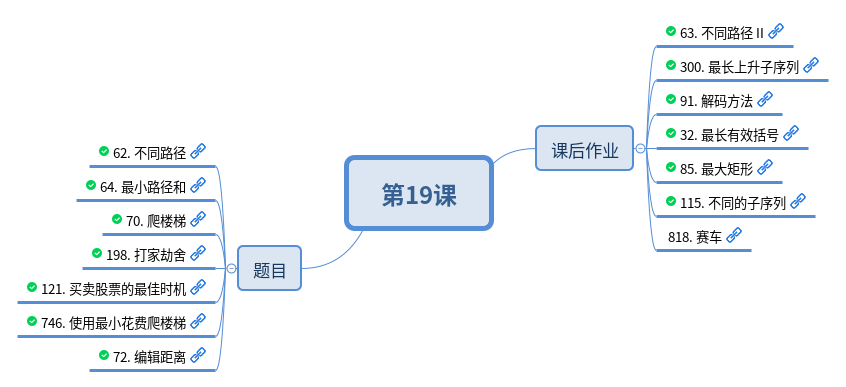
\includegraphics[width=130mm,height=60mm]{images/camp/第19课.png}

\subsubsection{题目}

\paragraph{实战题目}

\begin{itemize}
  \item \hyperref[leetcode:70]{70. 爬楼梯}
  \item \hyperref[leetcode:62]{62. 不同路径}
  \item \hyperref[leetcode:198]{198. 打家劫舍}
  \item \hyperref[leetcode:64]{64. 最小路径和}
  \item \hyperref[leetcode:121]{121. 买卖股票的最佳时机}
  \item \hyperref[leetcode:63]{63. 不同路径 II}
  \item \hyperref[leetcode:746]{746. 使用最小花费爬楼梯}
  \item \hyperref[leetcode:72]{72. 编辑距离}
\end{itemize}

\paragraph{课后作业}

\begin{itemize}
  \item \hyperref[leetcode:300]{300. 最长上升子序列}
  \item \hyperref[leetcode:91]{91. 解码方法}
  \item \hyperref[leetcode:32]{32. 最长有效括号}
  \item \hyperref[leetcode:85]{85. 最大矩形}
  \item \hyperref[leetcode:115]{115. 不同的子序列}
  \item \hyperref[leetcode:818]{818. 赛车}
\end{itemize}
